\scanpage{82}
Nous utiliserons \unsure{décidément|désormais} la base affine
$(s_0,s_1,s_{-1})$ pour identifier $E$ à $k^2$, donc

a) On choisit $s_0$ comme origine

b) On choisit
\[ \left\{\begin{aligned}e_1&=s_1-s_0\\
e_2&=s_{-1}-s_0\end{aligned}\right. \tag*{(15)} \]
comme vecteurs de base de l'espace des
translations $V$ de $E$, et

\deleted{\unsure{on}} c) on identifie $(x,y)\in k^2$ au point
$s_0+xe_1+ye_2$, i.e. on écrit
\[ (\unsure{x|a},y)=s_0+xe_1+ye_2. \]
Il y a lieu d'expliciter en termes de ces
coordonnées toutes les données précédentes.
\[ \left\{\begin{aligned} &s_0=(0,0),&s_1&=(1,0),&s_2&=(0,1)\\
&e_1=(1,0)&e_2&=(0,1)\end{aligned}\right. \]
Les autom affines $\sigma_0,\sigma_1$ sont donnés par leurs
valeurs sur $s_0,s_1,s_{-1}$. On a
\[ \left\{\begin{aligned}&\left\{\begin{aligned}\sigma_0s_0&=s_1\\
\sigma_0s_1&=s_0\\
\sigma_0s_{-1}&=s_2=s_0+(1+\alpha)e_1+(1+\beta)e_2\end{aligned}\right.\\
&\left\{\begin{aligned}\sigma_0 e_1&=-e_1\\
\sigma_0 e_2&=\deleted{\unsure{(1+\alpha)e_1+(1+\beta)e_2}}\inserted{\alpha e_1+(1+\beta)e_2}\end{aligned}\right.\end{aligned}\right. \tag*{(16)} \]

\figure{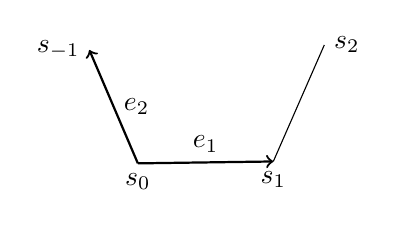
\begin{tikzpicture}[scale=.8]
\coordinate (o) at (0,0); \coordinate (a) at (2.15,.03); \coordinate (b) at (-.77,1.8); \coordinate (c) at (2.96,1.88);
\draw[->,thick] (o)--node[above] {$e_1$} (a); \draw[->,thick] (o)--node[right] {$e_2$} (b); \draw (a)--(c);
\node[below] at (o) {$s_0$}; \node[below] at (a) {$s_1$}; \node[left] at (b) {$s_{-1}$}; \node[right] at (c) {$s_2$};
\end{tikzpicture}}

\margin{[\,\uline{NB} on s'attend à $\left\{\begin{aligned}\beta&=0\ \text{i.e. }s_2-s_{\unsure{-1|+1}}\parallel e_1\\ \alpha&=\zeta+\zeta^{-1}=2\cos\theta\end{aligned}\right.$\,]}
% archive sheet number: 81
